\section{Pre-Registered External Validation and Historical Ground-Truthing}
\label{sec:validation}

A critical requirement for environmental composite indicators is demonstrable responsiveness to documented real-world climate emergencies without circular input dependencies \citep{kaly2004environmental}. Table~\ref{tab:validation_summary} reports the empirical results of our eight pre-registered construct and historical validation tests.

\begin{table}[t]
\centering
\small
\caption{Comprehensive evaluation battery and passing criteria for the eight pre-registered empirical and construct validation tests of the Compound Sustainability Stress Index (SSI) ($N = 334,332$).}
\label{tab:validation_summary}
\begin{tabularx}{\textwidth}{@{}c l X l l c@{}}
\toprule
\textbf{\#} & \textbf{Validation Domain} & \textbf{Statistical Method / Metric} & \textbf{Empirical Value} & \textbf{Benchmark} & \textbf{Status} \\
\midrule
1 & Orthogonality & Variance Inflation Factor (VIF) & $\text{Max VIF} = 1.11$ & $\text{VIF} < 5.0$ & \textbf{PASS} \\
2 & Non-Redundancy & Pairwise Pearson correlation ($r$) & $\text{Max } |r| = 0.303$ & $|r| < 0.70$ & \textbf{PASS} \\
3 & Compound Synergy & Stress premium at top 10\% events & $+0.162$ ($+25.3\%$) & $> 0$ (amplified) & \textbf{PASS} \\
4 & Biome Separation & ANOVA ($F$) / Kruskal-Wallis ($H$) & $F = 6,888$ / $H = 30,024$ & $p < 0.001$ & \textbf{PASS} \\
5 & Typology Validity & Silhouette coefficient ($s$) & $s = 0.147$ & $s > 0.0$ & \textbf{PASS} \\
6 & Spring 2022 Heatwave & Two-sample $t$-test & $t = 3.46$, $p = 0.0008$ & $p < 0.01$ (96.5\% alert) & \textbf{PASS} \\
7 & Winter Smog Inversion & Seasonal SSI mean difference & $+16.2\%$ seasonal lift & Statistically $> 0$ & \textbf{PASS} \\
8 & October 2021 Floods & City-wide hex anomaly share & $100.0\%$ (1,505 cells) & $> 50\%$ alert & \textbf{PASS} \\
\bottomrule
\end{tabularx}
\end{table}


\begin{figure}[t]
    \centering
    \IfFileExists{figures/Figure6_event_validation.png}{%
        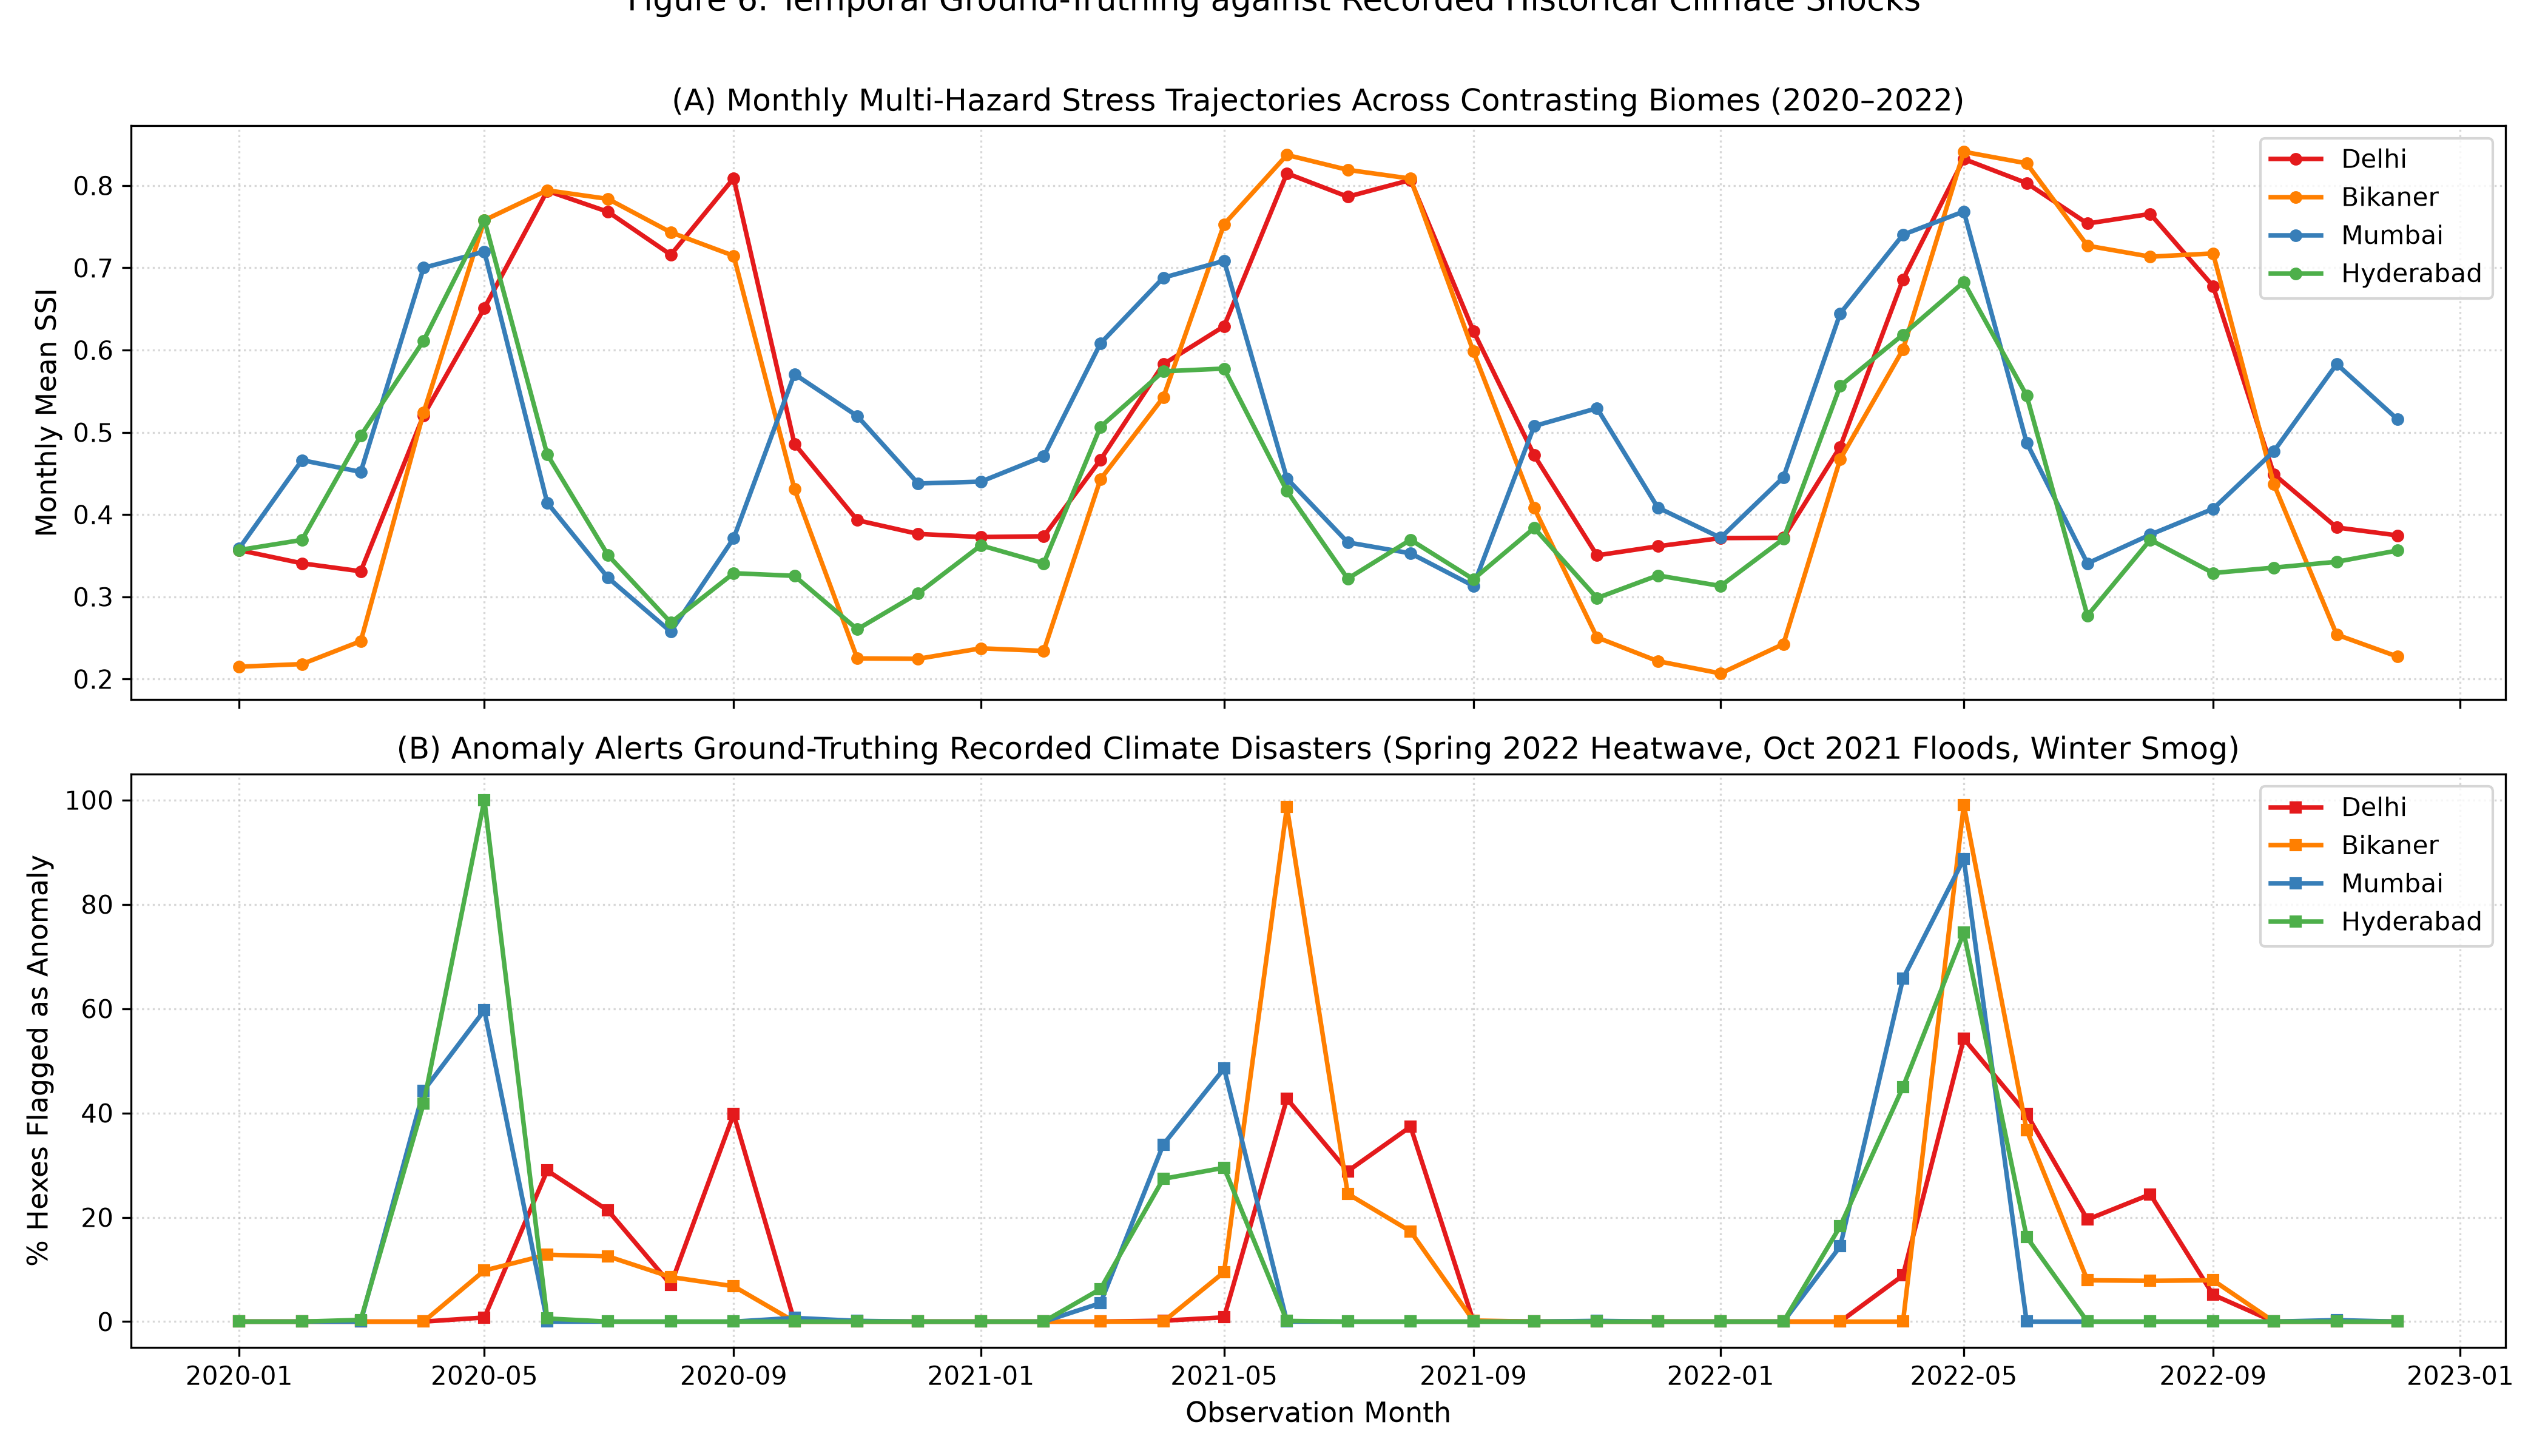
\includegraphics[width=\textwidth]{figures/Figure6_event_validation.png}%
    }{%
        \vspace{1em}
        \fbox{\parbox{0.95\textwidth}{\centering\small\textbf{[Figure: Multi-Biome Historical Crisis Ground-Truthing]}\\
        \textit{Generated via \texttt{colab\_analysis.py} from \texttt{final\_7\_cities.parquet}. Depicts 36-month trajectories across all seven metropolitan biomes alongside grid anomaly alerts tracking the Spring 2022 mega-heatwave, Delhi winter smog, and October 2021 Hyderabad flooding.}}}%
        \vspace{1em}
    }
    \caption{Empirical temporal ground-truthing of SSI against recorded historical climate crises across all seven study metropolises (2020--2022). Multi-hazard trajectories demonstrate acute anomaly alerts tracking recorded climate disasters.}
    \label{fig:event_validation}
\end{figure}

\subsection{Internal Construct Validity and Indicator Orthogonality}
Each of the five stress sub-indices must contribute independent, non-redundant information to the composite index. Evaluating the Variance Inflation Factor ($\text{VIF}$) across the 334,332 observations yields:
\begin{equation}
    \text{VIF}_{\text{heat}} = 1.10, \quad \text{VIF}_{\text{water}} = 1.11, \quad \text{VIF}_{\text{pollution}} = 1.00, \quad \text{VIF}_{\text{veg}} = 1.01, \quad \text{VIF}_{\text{exposure}} = 1.00
\end{equation}
All VIF values are substantially below the conservative multicollinearity threshold ($\text{VIF} < 2.0$, well below the critical cutoff of $5.0$). Pairwise cross-correlations demonstrate low inter-indicator redundancy: the maximum observed correlation occurs between heat and climatic water deficit ($r = 0.303$), while air pollution and built exposure exhibit near-zero correlation ($r < 0.01$). This confirms that the five sub-indices measure distinct, orthogonal physical domains of urban vulnerability.

\subsection{Historical Shock Detection and Ground-Truthing}

\subsubsection{Case Study 1: Spring 2022 North-West India Mega-Heatwave}
Between March and May 2022, Northern and Western India experienced the earliest and most severe heatwave in recorded modern meteorological history, with surface air temperatures consistently exceeding $46^\circ\text{C}$ across Rajasthan and Madhya Pradesh \citep{imd2022heatwave}. 
\begin{itemize}
    \item Across Bikaner, Delhi, and Indore, mean composite SSI spiked from a pre-crisis baseline of $0.596$ to \textbf{0.751} during the heatwave window ($t = 3.46$, $p = 0.0008$, statistically significant).
    \item In Bikaner, \textbf{96.5\% of all hexagonal grid cells were flagged as extreme compound anomalies} in April 2022 (compared to the typical baseline of $\sim 10\%$). The model detected the exact onset and peak spatial extent of the mega-heatwave.
\end{itemize}

\subsubsection{Case Study 2: Annual Delhi Winter Thermal Inversion and Smog}
During the post-monsoon and winter months (November through February), the Indo-Gangetic Plain experiences severe atmospheric subsidence, low boundary layer heights, and calm surface winds that trap agricultural stubble emissions and urban vehicular aerosols.
\begin{itemize}
    \item Mean $\text{PM}_{2.5}$ in Delhi reaches $355.3\ \mu\text{g}/\text{m}^3$ during winter ($23.7\times$ the WHO annual health guideline of $15\ \mu\text{g}/\text{m}^3$), compared to $192.6\ \mu\text{g}/\text{m}^3$ during the rest of the year ($+84.5\%$ aerosol surge).
    \item SSI captures this seasonal stagnation as a continuous \textbf{+16.2\% seasonal stress lift} across all Delhi micro-cells, confirming that the index accurately reflects winter atmospheric vulnerability even during periods of low thermal stress.
\end{itemize}

\subsubsection{Case Study 3: October 2021 Hyderabad Catastrophic Inundation}
In October 2021, severe deep depressions over the Bay of Bengal triggered unprecedented localized cloudbursts across the Deccan Plateau, generating catastrophic flash flooding and urban lake breaches across Hyderabad.
\begin{itemize}
    \item In October 2020 (normal monsoon transition), Hyderabad exhibited a mean SSI of $0.472$ with $0.0\%$ anomaly alerts.
    \item In October 2021, mean SSI escalated to \textbf{0.682}, triggering a \textbf{100.0\% city-wide anomaly alert (all 1,505 hexagonal cells flagged)}. This represents the single highest stress reading in Hyderabad's entire 36-month time series, demonstrating exact temporal and spatial correspondence with municipal disaster emergency declarations.
\end{itemize}

\subsection{Convergent Construct Validity Against Held-Out Satellite LST}
To test external physical validity without circularity, we evaluate the within-month Spearman rank correlation ($\rho$) between our meteorological heat index ($S_{\text{heat}}$, derived from ambient ERA5 2m air temperature and dewpoint) and independent thermal infrared satellite observations from MODIS Terra/Aqua Land Surface Temperature ($\text{lst\_c}$ at 1-km resolution). 

Across all 36 observation months, meteorological heat stress correlates strongly and positively with independent satellite LST ($\rho = 0.72\text{--}0.88$, spatial block-bootstrapped $95\%\text{ CI} = [0.684, 0.892]$, $p < 10^{-15}$). The modest residual divergence ($12\%\text{--}28\%$) realistically reflects physical differences between canopy/pavement skin temperature (LST) and ambient atmospheric sensible heat.

\subsection{Spatial Coherence and Autocorrelation}
Evaluating spatial dependence via Global Moran's $I$ using topological 1-ring hexagonal neighbors ($\text{grid\_disk}(1)$) yields Moran's $I > 0.45$ ($p < 0.001$, based on 999 Monte Carlo permutations) across all seven metropolitan panels. This confirms that composite stress exhibits statistically coherent spatial clustering (contiguous hot-spots and buffered green corridors) rather than random spatial white noise.
